%%% PGDAY FR 2012
%%%
%%% Implementing High Availability
%%%
%%% How to implement PostgreSQL in a demanding project, what are the
%%% different technical offerings good for? All you wanted to know about
%%% replication and never dared to ask.
%%%
%%% PostgreSQL includes several High Availability solution, some replication
%%% solutions, and some external Open Source projects complement the
%%% offering. When to use which project and what for? This talk will present
%%% the usual needs you want to address in a medium size project and how to
%%% use several replication solutions to implement them.

\documentclass[english]{beamer}
\usepackage[utf8]{inputenc}
%%\usepackage[latin9]{inputenc}
\usepackage[T1]{fontenc}
\usepackage{babel}
\usepackage{eurosym}

\usepackage{beamerthemesplit}
%% \usetheme{Warsaw}
\usetheme{Frankfurt}
\beamertemplatetransparentcovered

\title{Implementing High Availability}
\subtitle{with PostgreSQL}
\author{Dimitri Fontaine \newline\tiny{\texttt{dimitri@2ndQuadrant.fr}}}
\date{25 Oct. 2012}
\logo{
\includegraphics[height=0.4cm]{2ndQuadrant-cross.png}}

\begin{document}

\frame{\titlepage}

\section{Agenda}
\subsection{whoami}
\frame{\tableofcontents[currentsection]}

\begin{frame}[fragile]
  \frametitle{Dimitri Fontaine}

  \begin{center}
    \textbf{2ndQuadrant France}
    \linebreak
    PostgreSQL Major Contributor
  \end{center}
  \linebreak

\begin{columns}[c]
\column{.75\textwidth} 

  \begin{itemize}
   \item<1-> \texttt{pgloader}, \texttt{prefix}, \texttt{skytools}, \texttt{debian}, …
   \item<1-> \texttt{\textbf{CREATE EXTENSION}}
   \item<2-> \texttt{\textbf{CREATE EVENT TRIGGER}}
   \item<2-> \textit{Bi-Directional Replication}
   \item<3-> \textit{Partitioning}
  \end{itemize}  

\column{.25\textwidth}
\begin{center}
  
\includegraphics[height=5em]{bulle-blue-icon.png}
\end{center}
\end{columns}
\end{frame}

\begin{frame}[fragile]
  \frametitle{Proven Architectures, implemented lots at Hi-Media}

  \center{\textbf{Hi-Media} (turnover scale: 200 millions \euro)}

\begin{columns}[c]
\column{.75\textwidth} 

   \onslide<2->{\center{3 different activities to get money from the web}}

  \begin{itemize}
   \item<2-> Allopass, HiPay : internet (micro) payment
   \item<2-> Telecom Service
   \item<2-> Advertising
  \end{itemize}  

  \onslide<3->{\center{PostgreSQL is the heart of the technical platform}}

  \begin{itemize}
  \item<4-> Business needs compliance
  \item<4-> Capacity to adapt to changes
  \end{itemize}  

\column{.25\textwidth}
\begin{center}
  
\includegraphics[height=7em]{agenda.jpg}
\end{center}
\end{columns}
\end{frame}

\begin{frame}[fragile]
  \frametitle{PostgreSQL: Your data is our job}

  \begin{center}
    How to ensure \emph{both} \textit{duralibity} and \textit{availability}
    of your data?
  \end{center}
  \linebreak

\begin{columns}[c]
\column{.75\textwidth} 

  Usual needs :

  \begin{itemize}
   \item<2-> Reliability
   \item<2-> Stability
   \item<2-> Performances
   \item<3-> Growth capacity (think commercial success)
   \item<3-> Continuity and Innovation
  \end{itemize}  

\column{.25\textwidth}
\begin{center}
  
\includegraphics[height=7em]{agenda.jpg}
\end{center}
\end{columns}
\end{frame}

\subsection{Availability, Duralibity}
\frame{\tableofcontents[currentsubsection]}

\begin{frame}
  \frametitle{Glossary}
  
  \center{Some vocabulary}
  \linebreak
  \linebreak

\begin{columns}[c]
\column{.75\textwidth} 

  \begin{itemize}
    \item<3,4,6> Availability \only<4->{\textit{of services or of data?}}
    \item<2,6> Duralibity (ACI\alert{D})
    \item<5,6> Architectures
    \item<1,6> Replications
  \end{itemize}  

\column{.25\textwidth}

\includegraphics[height=6em]{glossaire.jpg}
\end{columns}
\end{frame}

\subsection{Architectures and Replications}

\begin{frame}[fragile]
  \frametitle{Needs first}

  \center{Needs evolve, solutions must adapt}
  \linebreak

\begin{columns}[c]
\column{.75\textwidth} 

\begin{itemize}
  \item<1-> Start simple
  \item<1-> Some first classic steps
  \item<2-> High Availability of Data
  \item<2-> High Availability of Services
  \item<3-> Read Only Load Balancing
  \item<3-> Read Write Load Balancing
\end{itemize}

\column{.25\textwidth}
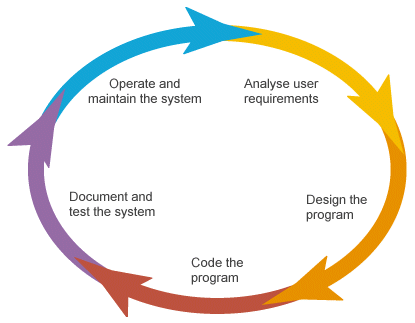
\includegraphics[height=5em]{development_life_cycle.png}
\end{columns}
\end{frame}

\begin{frame}[fragile]
  \frametitle{Let's start simple}

  \center{Our projet life cycle}
  \linebreak

\begin{columns}[c]
\column{.75\textwidth} 

  Let's start with the example of a quite simple project released as a web
  application seeing its needs evolve with its success.

  \center{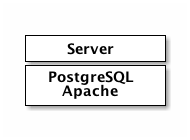
\includegraphics[height=1in]{archi_v1.png}}  

\column{.25\textwidth}
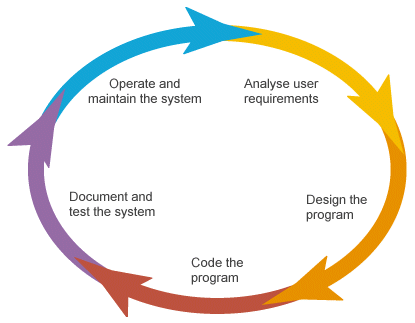
\includegraphics[height=5em]{development_life_cycle.png}
\end{columns}
\end{frame}

\section{Isolate Services}
\subsection{Trafic growth}
\frame{\tableofcontents[currentsubsection]}

\begin{frame}[fragile]
  \frametitle{Scaling out 101}

  \center{Services Availability}
  \linebreak
  \linebreak

\begin{columns}[c]
\column{.65\textwidth} 

  \begin{itemize}
   \item<1-> Front servers are \textit{stateless}
   \item<2-> Watch out for \texttt{max\_connections}
   \item<2-> Don't you use persistent connections!
   \item<3-> \texttt{pgbouncer}
  \end{itemize}  

\column{.35\textwidth}

\includegraphics[height=4em]{bouncer.png}
\end{columns}
\end{frame}


\frame{
  \frametitle{Scaling out 101}

  \center{Using more than a single server and a connection pool}

\begin{center}
  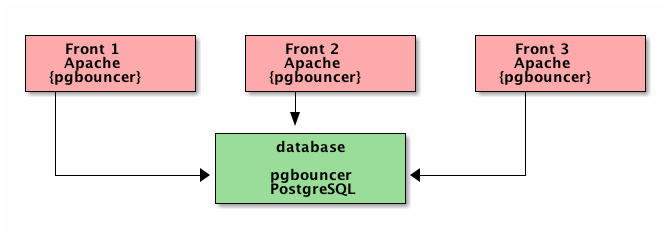
\includegraphics[height=1.3in]{archi_v2.png}
\end{center}  
}

\begin{frame}[fragile]
  \frametitle{pgbouncer}

  \center{\texttt{pgbouncer} is able to reuse client \textbf{and} server
    side connections.}

  \only<1>{
    \begin{center}
      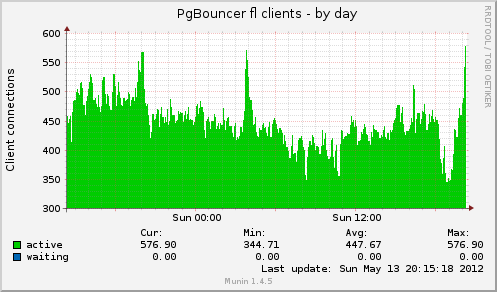
\includegraphics[height=2in]{pgbouncer_db_fl_pools_cl-day.png}
    \end{center}
  }
  \only<2>{
    \begin{center}
      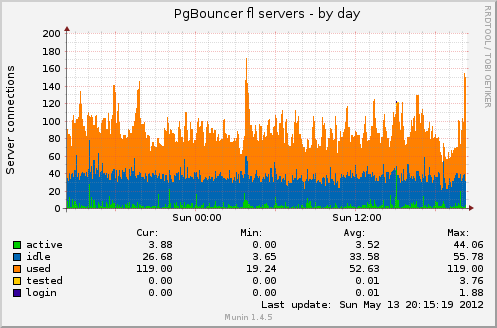
\includegraphics[height=2in]{pgbouncer_db_fl_pools_sv-day.png}
    \end{center}
  }
\end{frame}

\section{Durability}
\subsection{Data Durability}
\frame{\tableofcontents[currentsubsection]}

\begin{frame}[fragile]
  \frametitle{Getting serious: backups}

  \center{Backup Strategy is the single most important step towards data availability}

\begin{columns}[c]
\column{.65\textwidth} 

  \begin{itemize}
   \item<1-> Nightly \texttt{pg\_dump -Fc}
   \item<1-> Don't forget \texttt{pg\_dumpall --globals-only}
   \item<2-> Data Retention
   \item<2-> 7 days of nightly backups
   \item<2-> 7 weeks of weekly backups
   \item<2-> 12 months of monthly backups
   \item<3-> 30 years of yearly backups?
  \end{itemize}  

\column{.35\textwidth}
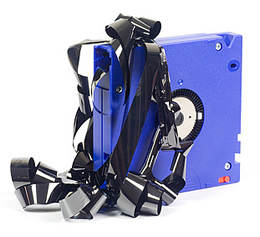
\includegraphics[height=7em]{online-backup.jpg}
\end{columns}
\end{frame}

\begin{frame}[fragile]
  \frametitle{Failover, 101}

  \center{\texttt{pg\_dump}, \texttt{pg\_restore}}
  \linebreak
  \linebreak

\begin{columns}[c]
\column{.75\textwidth} 

  \begin{itemize}
    \item<1-> protection against \textit{errors and omissions}
    \item<1-> beware of restoring time
    \item<2-> still a must have for data \textbf{durability}
    \item<2-> what about data \textbf{availability}?
  \end{itemize}

\column{.25\textwidth}
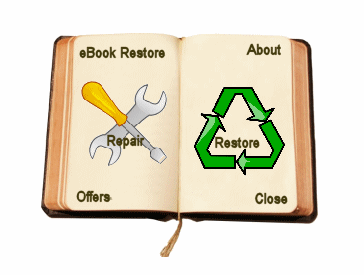
\includegraphics[height=7em]{restore.png}
\end{columns}
\end{frame}

\subsection{Data Availability}
\frame{\tableofcontents[currentsubsection]}

\begin{frame}[fragile]
  \frametitle{Failover, 201}

  \center{Using physical backups and \textit{Point In Time Recovery}}

\begin{columns}[c]
\column{.65\textwidth} 

  \begin{itemize}
   \item<1-> \alert{Point In Time Recovery}, 8.1
   \item<2-> \textit{warm standby}, 8.2
   \item<3-> Archiving and \textit{crash recovery}
   \item<3-> \texttt{archive\_command}
   \item<3-> \texttt{restore\_command}
   \item<4-> \texttt{walmgr.py}, {\texttt{WAL-E}
  \end{itemize}  

\column{.35\textwidth}

\includegraphics[height=6em]{pitr.png}
\end{columns}
\end{frame}

\frame{
  \frametitle{Warm Standby}

  \center{Implementing \textit{Warm Standby}}

\begin{center}
  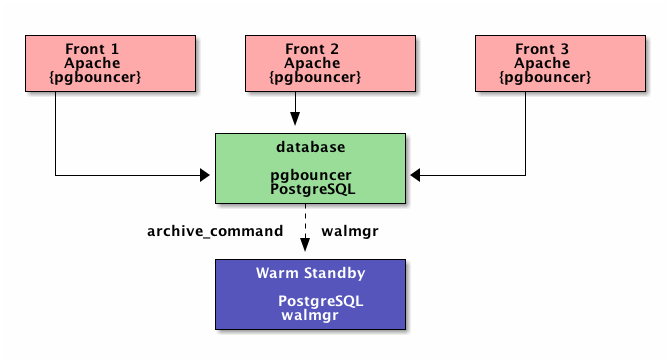
\includegraphics[height=2.1in]{archi_v3.png}
\end{center}    
}

\section{Availability}
\subsection{Services Availability}
\frame{\tableofcontents[currentsubsection]}

\begin{frame}[fragile]
  \frametitle{Application Split}

  \center{When you have separate \textit{backoffice} and \textit{production} requirements}
  \linebreak

\begin{columns}[c]
\column{.65\textwidth} 

  \begin{itemize}
   \item<1-> Cross replication
   \item<2-> Slony, \textbf{Londiste}, Bucardo
   \item<3-> Specific processing, \textit{batches}
   \item<3-> \textIt{Off-line} processing
   \item<3-> Still \textit{Transactional} processing
   \item<4-> Skytools comes with \alert{\textbf{PGQ}}
  \end{itemize}  

\column{.35\textwidth}

\includegraphics[height=6em]{cross-replication.jpg}
\end{columns}
\end{frame}

\frame{
  \frametitle{Application Split}

  \center{Implementing \textit{londiste} and \textit{PGQ}}

\begin{center}
  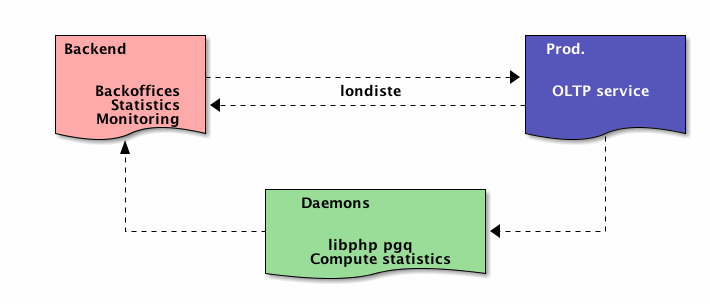
\includegraphics[height=1.7in]{archi_v4.png}
\end{center}    
}

\begin{frame}[fragile]
  \frametitle{Queueing with \textit{PGQ}}

  \center{\textit{Off-line} processing is better done with \texttt{PGQ}}
  \linebreak

\begin{columns}[c]
\column{.6\textwidth} 

  \begin{itemize}
   \item<1-> Mainly written in \texttt{PLpgSQL} (and \texttt{C})
   \item<1-> Client \textit{API} for \texttt{python}
   \item<1-> and \texttt{PHP}
   \item<2-> some work is happening for \texttt{Java}
   \item<3-> \textbf{Cooperative Worker} (Skytools 3)
  \end{itemize}  

  \onslide<4->{\center{\texttt{PGQ}: Stable, Reliable, Easy to monitor}}

\column{.4\textwidth}

\includegraphics[height=9em]{drop-queue.png}
\end{columns}
\end{frame}

\begin{frame}[fragile]
  \frametitle{Disaster Recovery and Service Continuity}

  \center{PostgreSQL 9.1 offers \textit{Synchronous Replication} and \textit{Hot Standby}}
  \linebreak

\begin{columns}[c]
\column{.6\textwidth} 

  \begin{itemize}
   \item<1-> \alert{Hot Standby}
   \item<2-> \textit{(A)}Synchronous Replication
   \item<2-> Standby connects with \texttt{libpq}
   \item<3-> \texttt{recovery.conf}
   \item<3-> Continue Archiving
   \item<3-> Switchabe \textbf{per transaction}
   \item<4-> Good performance level
  \end{itemize}  

\column{.4\textwidth}

\includegraphics[height=9em]{bits.jpeg}
\end{columns}
\end{frame}

\frame{
  \frametitle{Disaster Recovery and Service Continuity}
  \center{Implementing Hot Standby}
  
\begin{center}
  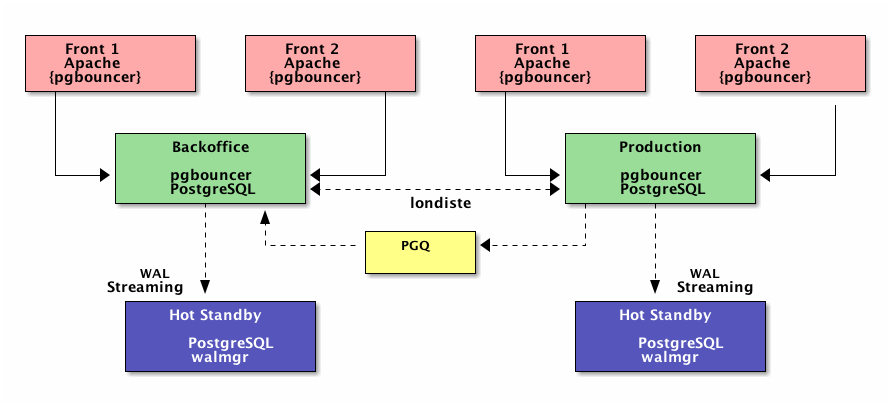
\includegraphics[height=1.9in]{archi_v5.png}
\end{center}
}

\subsection{Sharding}
\frame{\tableofcontents[currentsubsection]}

\begin{frame}[fragile]
  \frametitle{Scaling Writes}

  \center{\texttt{PL/proxy}}
  \linebreak
  \linebreak

\begin{columns}[c]
\column{.6\textwidth} 

  \begin{itemize}
   \item<1-> \textit{Scale-up} or \textit{Scale-out} ?
   \item<2-> \textit{Remote Procedure Call}
   \item<3-> \textit{Sharding}
   \item<3-> Distributed database
   \item<4-> Autonomous Transactions
   \item<5-> \textbf{Stored Procedures}
  \end{itemize}  

\column{.4\textwidth}

\includegraphics[height=9em]{distribution.jpg}
\end{columns}
\end{frame}

\begin{frame}[fragile]
  \frametitle{\texttt{PL/Proxy}}
  
  \center{Installing \texttt{plproxy}}

\begin{columns}[c]
\column{.6\textwidth} 

  \begin{example}[install.sql]
\begin{verbatim}
=# create extension plproxy;
=# create extension hashlib;
\end{verbatim}
  \end{example}

\column{.4\textwidth}

\includegraphics[height=9em]{distribution.jpg}
\end{columns}
\end{frame}

\begin{frame}[fragile]
  \frametitle{\texttt{PL/Proxy}}

  \textit{pl/proxy} is the integrated sharding layer. Now you have to write
  all your SQL in server side functions.

  \begin{example}[admin/change\_group\_status.sql]
\begin{verbatim}
create or replace function admin.change_group_status
(
    user_name text, status integer
)
returns void as $BODY$
    CLUSTER 'fl_cluster';
    RUN ON hash_string(user_name, 'lookup3le');
$BODY$;
\end{verbatim}
  \end{example}
\end{frame}

\begin{frame}[fragile]
  \frametitle{Distributed Sequences 1/2}

  Same schema on every node, best to avoid overlapping sequences.

\begin{columns}[c]
\column{.6\textwidth} 

  \begin{example}[distributing sequence]
\begin{verbatim}
ALTER SEQUENCE foo_id_seq
  INCREMENT BY 16;
\end{verbatim}
  \end{example}

\column{.4\textwidth}

\includegraphics[height=9em]{distribution.jpg}
\end{columns}
\end{frame}

\begin{frame}[fragile]
  \frametitle{Distributed Sequences 2/2}

  Same schema on every node, best to avoid overlapping sequences.

\begin{columns}[c]
\column{.6\textwidth} 

  \begin{example}[distributing sequence]
\begin{verbatim}
ALTER SEQUENCE foo_id_seq
      MINVALUE 297000000000000000
      MAXVALUE 297999999999999999;
\end{verbatim}
  \end{example}

\column{.4\textwidth}

\includegraphics[height=9em]{distribution.jpg}
\end{columns}

  \onslide<2->{\center{\url{http://www.fotolog.com/<user>/297000000000017139/}}}
\end{frame}

\frame{
  \frametitle{Scaling Writes}
  \center{Implementing \texttt{plproxy}}

  \only<1>{
    \begin{center}
      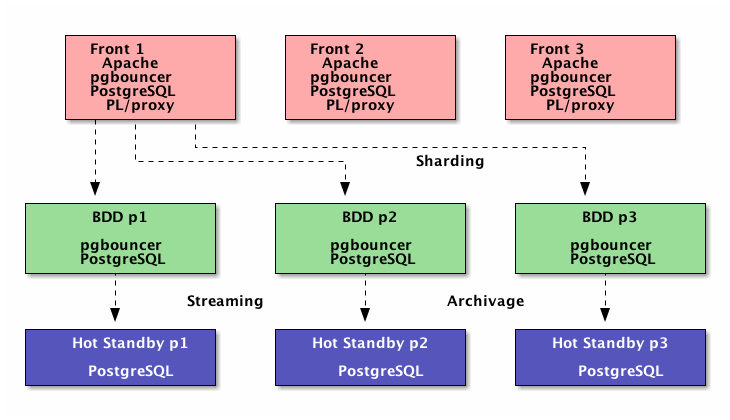
\includegraphics[height=1.9in]{archi_v6.png}
    \end{center}
  }
  \only<2>{
    \begin{center}
      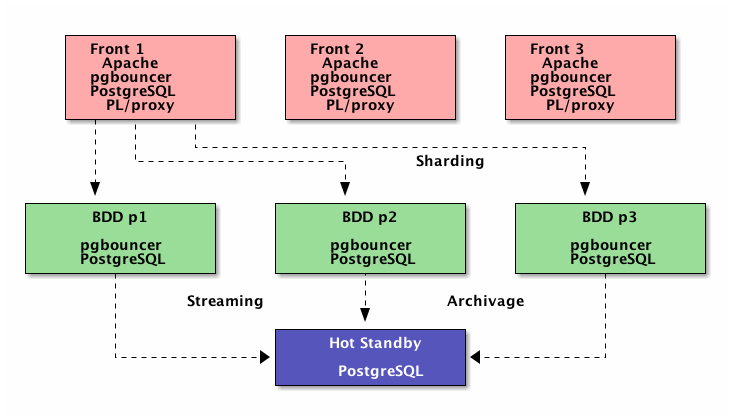
\includegraphics[height=1.9in]{archi_v7.png}
    \end{center}
  }
}

\section{Conclusion}
\subsection{PostgreSQL Replication: Looking back, looking forward}
\frame{\tableofcontents[currentsubsection]}

\begin{frame}[fragile]
  \frametitle{Distributed High Availability}

  \center{Retrospective and Future of PostgreSQL Replication}
  \linebreak

\begin{columns}[c]
\column{.55\textwidth} 

  \begin{itemize}
   \item<1-> \textbf{8.1}, PITR
   \item<2-> \textbf{8.2}, Warm Standby
   \item<3-> \textbf{8.3}, \texttt{pg\_standby}
   \item<4-> \textbf{9.0}, Hot Standby
   \item<5-> \textbf{9.1}, Synchronous Replication
   \item<6-> \textbf{9.2}, Cascading Replication
   \item<7-> \textbf{9.3}, \alert{Bi-Directional Replication}
  \end{itemize}  

\column{.45\textwidth}

\includegraphics[height=9em]{bdr.png}
\end{columns}
\end{frame}

\subsection{Questions}

\frame{
  \frametitle{Questions ?}

\begin{center}
  Meet with us on the booth, join us in the \textit{Hallway Track}!
  \linebreak
  \linebreak

  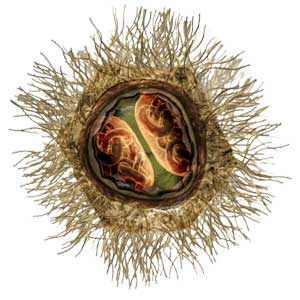
\includegraphics[height=9em]{in-core-replication.jpg}
\end{center}
}

\end{document}
